\documentclass[sigconf,review,anonymous]{acmart}

\makeatletter
\@ACM@balancefalse
\makeatother
\let\Bbbk\relax
\usepackage{amsmath,amssymb,mathtools}
\usepackage{amsthm}
\usepackage{booktabs}
\usepackage{multirow}
\usepackage{tabularx}
\usepackage{array}
\usepackage{float}
\usepackage{placeins}
\usepackage{tikz}
\usepackage{pgfplots}
\pgfplotsset{compat=1.18}
\usepackage{listings}
\usepackage{adjustbox}
\AtBeginDocument{%
  \setlength{\textfloatsep}{10pt plus 2pt minus 2pt}%
  \setlength{\intextsep}{9pt plus 2pt minus 2pt}%
  \setlength{\dbltextfloatsep}{12pt plus 2pt minus 2pt}%
}

% acmart pre-loads natbib, hyperref, xcolor, graphicx, microtype, geometry, fontenc, inputenc.
% Do not re-load them here.

\hfuzz=2pt
\emergencystretch=3em
\hbadness=10000
\vbadness=10000

\lstset{
  basicstyle=\ttfamily\footnotesize,
  breaklines=true,
  frame=single,
  language=Python,
  keywordstyle=\color{blue},
  commentstyle=\color{green!50!black},
  stringstyle=\color{red!70!black},
  showstringspaces=false
}

%==============================================================================
% ACM CONFERENCE METADATA
%==============================================================================
\acmConference[SACMAT '27]{The 32nd ACM Symposium on Access Control Models and Technologies}{June 2027}{To be announced}
\acmYear{2027}
\copyrightyear{2027}
\acmISBN{978-1-4503-XXXX-X/27/06}
\acmDOI{10.1145/XXXXXXX.XXXXXXX}
\setcopyright{acmlicensed}

%==============================================================================
% CCS CONCEPTS (REQUIRED BY ACM)
%==============================================================================
\begin{CCSXML}
<ccs2012>
   <concept>
       <concept_id>10002978.10003006.10003013</concept_id>
       <concept_desc>Security and privacy~Access control</concept_desc>
       <concept_significance>500</concept_significance>
       </concept>
   <concept>
       <concept_id>10002978.10003006.10003007</concept_id>
       <concept_desc>Security and privacy~Authorization</concept_desc>
       <concept_significance>300</concept_significance>
       </concept>
   <concept>
       <concept_id>10010147.10010178.10010224</concept_id>
       <concept_desc>Computing methodologies~Multi-agent systems</concept_desc>
       <concept_significance>300</concept_significance>
       </concept>
   <concept>
       <concept_id>10002978.10003001.10003003</concept_id>
       <concept_desc>Security and privacy~Logic and verification</concept_desc>
       <concept_significance>100</concept_significance>
       </concept>
 </ccs2012>
\end{CCSXML}

\ccsdesc[500]{Security and privacy~Access control}
\ccsdesc[300]{Security and privacy~Authorization}
\ccsdesc[300]{Computing methodologies~Multi-agent systems}
\ccsdesc[100]{Security and privacy~Logic and verification}

\keywords{access control, RBAC, ABAC, typed predicates, Model Context Protocol, agentic AI, LLM safety, policy enforcement, zero trust}

\title{PALADIN: Policy-Aware Layered Agentic Decision Intelligence over the Model Context Protocol}

%==============================================================================
% AUTHORS (ANONYMISED FOR DOUBLE-BLIND REVIEW)
%==============================================================================
% The "anonymous" class option suppresses author names, affiliations, and emails
% in the rendered PDF. Author metadata is retained below for the camera-ready.
\author{Author One}
\affiliation{%
  \institution{Anonymous Institution}
  \city{Anonymous City}
  \country{Anonymous Country}
}
\email{anon1@example.com}

\author{Author Two}
\affiliation{%
  \institution{Anonymous Institution}
  \city{Anonymous City}
  \country{Anonymous Country}
}
\email{anon2@example.com}

\author{Author Three}
\affiliation{%
  \institution{Anonymous Institution}
  \city{Anonymous City}
  \country{Anonymous Country}
}
\email{anon3@example.com}

\renewcommand{\shortauthors}{Anon.}

\begin{document}

%==============================================================================
% ABSTRACT
%==============================================================================
\begin{abstract}
\begin{sloppypar}
Autonomous LLM agents now invoke external tools through the Model Context Protocol (MCP), turning every tool call into an authorisation decision the protocol itself does not make. We argue this is an \emph{access-control} problem---and that the field has been answering the wrong question: \emph{semantic correctness is not authorisation correctness}. The tools that best accomplish a task can be exactly the ones an agent is not permitted to use, while a poorly-chosen bundle may be perfectly admissible. We introduce \textbf{PALADIN}, a deterministic invocation-time authorisation pipeline (SPIFFE/SPIRE identity, RBAC, ABAC, then TRAC), whose novel stage is \textbf{TRAC}---a \emph{task-relational} admission primitive that authorises an invocation on the coherence between the task and its proposed action-set.

Our central result: this deterministic floor holds worst-case SecFail to a fixed $10.3\%$, identical across every model. On ASTRA~\cite{elhelou2025astra}, an agentic tool-selection safety benchmark, six LLMs from three vendors used \emph{alone} as admission controllers wrongly admit $27$--$67\%$ of unsafe tool calls---unreliable, with no monotonic improvement across newer or stronger models. Composed \emph{behind} the floor, the \emph{same} models all converge to at most $7.5\%$. Around this we build a measurement framework for layered authorisation: it separates an LLM \emph{judging} a candidate bundle from one \emph{generating} it, and shows that na\"ive attribution misranks which policy layers matter. The floor guards \emph{semi-honest} mis-scoping (the common case) at a bounded false-block cost; it composes with prompt-injection defences for adversarial input and needs no bespoke runtime (verified OPA/Rego parity). All policies, logs, and scripts are released.
\end{sloppypar}
\end{abstract}

\maketitle

%==============================================================================
% SECTION 1: INTRODUCTION
%==============================================================================
\section{Introduction}
\label{sec:introduction}

\subsection{Motivation}
\label{sec:motivation}

LLM agents that autonomously select and invoke external tools have proliferated across enterprise and consumer domains~\cite{wang2024survey, xi2025rise}, building on tool-augmented language models~\cite{schick2023toolformer} and ReAct-style reasoning-and-acting loops~\cite{yao2023react}. They now standardise on the Model Context Protocol (MCP)~\cite{anthropic2024mcp} as the de facto tool-invocation interface. MCP deployments typically assume a trusted execution environment with no native identity verification, permission scoping, or deterministic predicate evaluation. The security gap is consequential: an agent tasked with ``investigating anomalous metrics'' might autonomously select tools that modify production alert rules, mutate database state, or initiate financial transactions far outside its intended mission. Recent analyses catalogue 16 MCP-lifecycle threat categories~\cite{gupta2025security} and document exploits including credential theft, tool poisoning, and remote code execution~\cite{jamshidi2025securing}.

Existing LLM-security work addresses fragments. Prompt-injection defences~\cite{liu2024formalizing, zhan2024injecagent} target adversarial reasoning manipulation; output filters such as Llama Guard~\cite{inan2023llamaguard} constrain generation content; agent-safety benchmarks~\cite{zhang2024agentsafetybench, yuan2024rjudge} evaluate behaviour in controlled environments. None reasons about the security properties of \emph{individual tool invocations} within a multi-domain operational context. Chu et al.~\cite{chu2026stateless} identify a layered attack-surface model but provide no enforcement mechanism; we instantiate one as a staged invocation-time pipeline.

This exposes a reframing the agentic-AC literature has largely missed: \emph{task-tool semantic correctness is not authorisation correctness}. A bundle a task-tool benchmark scores as ``correct''---the tools that best accomplish the task---may still be \emph{inadmissible} under the agent's role, attribute, and task-coherence constraints; conversely a benchmark-incorrect bundle may be perfectly admissible. Authorising agentic tool use is therefore an access-control problem, not a retrieval-accuracy one. It needs an enforcement primitive that conditions on the task$\leftrightarrow$bundle relation---a relation outside the \emph{conventional} attribute vocabulary of RBAC and ABAC, yet, like ReBAC and Purpose-BAC, enforceable on a standard policy engine once derived (\S\ref{sec:substrate_portability}).

\subsection{Contributions}
\label{sec:contributions}

Our primary contribution is an \emph{access-control} one: we recast agentic tool invocation as an authorisation problem (semantic correctness $\neq$ authorisation correctness) and introduce a \emph{task-relational} admission primitive---\textbf{TRAC} (task-relational access control)---that authorises on the discriminating signal conventional access control omits: the coherence between the task and its proposed action-set. We do \emph{not} claim a new formal model: TRAC needs no new rule-engine machinery and runs as rules-as-data on a commodity engine (verified OPA/Rego parity, \S\ref{sec:substrate_portability}). The novelty is the \emph{reframing}, the \emph{leak-free derivation} of that coherence attribute at invocation time (consuming no ground-truth label, \S\ref{sec:domain_inference}), a \emph{measurement methodology} for layered authorisation (how a deterministic policy stack and LLM judgement compose), and the empirical demonstration that measured semantic coherence is a reliable, load-bearing authorisation attribute---all realised in \textbf{PALADIN} (Policy-Aware Layered Agentic Decision Intelligence), our deterministic invocation-time authorisation pipeline (SPIFFE/SPIRE identity $\to$ RBAC $\to$ ABAC $\to$ a fact transformer $\to$ TRAC) in which TRAC is the novel stage. Concretely:

\begin{enumerate}
  \item A \textbf{methodology for measuring layered authorisation}: a dual-mode validation/selection protocol (the LLM \emph{judging} a candidate bundle vs.\ \emph{generating} one) that most benchmarks conflate; two metric conventions (security- vs.\ permissivity-view) that disagree on layer importance and must be reported jointly; paired task-level bootstrap CIs on layer marginals; and a dataset-ceiling analysis bounding exact-match at $30$--$40\%$ (\S\ref{sec:methodology},~\ref{sec:conventions},~\ref{sec:ceiling}).

  \item A \textbf{task-relational admission primitive, TRAC}: it authorises an invocation on the \emph{measured coherence between the task and the proposed bundle}---in-domain coverage, mutation safety, task--tool relevance---a task$\leftrightarrow$bundle relation outside conventional RBAC/ABAC vocabulary and distinct from the workflow (TBAC~\cite{thomas1997tbac}), entity (ReBAC~\cite{fong2011rebac}), and \emph{declared}-purpose (Purpose-BAC~\cite{byun2005purpose}) axes. Derived by a fact transformer, it consumes \emph{no ground-truth label} (BM25 domain inference, \S\ref{sec:domain_inference}) and is enforceable on commodity engines (OPA/Rego parity, \S\ref{sec:substrate_portability}); we claim an empirical, load-bearing authorisation signal, not a new formal model. Every decision recomputes from the released logs without LLM calls.

  \item A \textbf{deterministic security floor whose \emph{magnitude} we measure}: conditioning on the bundle not the model, the stack returns a bit-identical profile ($F_1\!=\!0.848$, SecFail $10.3\%$) for every model---the empirical content is the floor's magnitude, not the by-construction invariance. LLM-only $F_1$ ranges $0.28$ on the same inputs; composing the model's verdict behind the floor sharpens SecFail to $2.1\%$ (gpt-4o) and never exceeds the floor. A blind cross-vendor panel (Claude Opus 4.8, Sonnet 4.6, Gemini 2.5 Pro; all $6{,}942$ rows) converges to SecFail $\leq\!7.5\%$ (\S\ref{sec:stack_guarantee},~\ref{sec:newer_not_better}).

  \item \textbf{Complementary layers, measured two ways} (paired CIs): drop-one marginals are $-20.7$pp (RBAC) and $-12.0$pp (TRAC)---each individually load-bearing---while ABAC's is only $-0.9$pp (it overlaps RBAC) yet load-bearing when RBAC is absent (successive $-23.4$pp). Under a label defined independently of every policy artefact TRAC's marginal becomes the \emph{largest} (\S\ref{sec:reversal}); the successive/drop-one gap exposes a first-firing attribution pitfall (\S\ref{sec:per_domain}).

  \item \textbf{Attribution paradox and corroborated coverage}: (a) first-firing denial attribution misleads---RBAC claims $82\%$ of denials, yet ABAC (claiming $4\%$) carries the \emph{largest} successive marginal ($-23.4$pp)---a pitfall in much of the agent-safety literature; and (b) \emph{corroborated coverage} recovers legitimate work at near-zero security cost. We also reproduce ASTRA's LLM-ResM~\cite{elhelou2025astra} under a stricter per-bundle protocol (\S\ref{sec:attribution_paradox},~\ref{sec:corroborated}).
\end{enumerate}

\noindent\textbf{What this paper is not.} PALADIN is a security-first invocation-time floor, not an end-to-end agent-security solution: prompt-injection, tool-output exfiltration, MCP supply-chain, and side-channel attacks are out of scope and compose with it (\S\ref{sec:deployment_envelope}).

%==============================================================================
% SECTION 2: RELATED WORK
%==============================================================================
\section{Related Work}
\label{sec:related}

\subsection{Access Control, Policy Languages, and Task-Tool Benchmarks}
\label{sec:access_control}

Five decades of access-control foundations span lattice models~\cite{bell1973secure}, RBAC~\cite{sandhu1996role,ferraiolo2001proposed}, ABAC~\cite{hu2014guide}, and policy languages with decidable analysis (Cedar~\cite{cutler2024cedar}, XACML~\cite{oasis2013xacml}, Margrave~\cite{fisler2005verification}). These were designed for human principals on static boundaries; agents construct invocations dynamically via probabilistic reasoning, span multiple domains per task, and produce confidence scores carrying security-relevant signal.

Two AC lineages model structure beyond the subject and are the natural reference points for a ``task-relational'' claim. \emph{Task-Based Access Control} (TBAC)~\cite{thomas1997tbac} ties permission \emph{activation} to a task's workflow lifecycle---permissions are granted and revoked just-in-time as a task advances through its steps. \emph{Relationship-Based Access Control} (ReBAC)~\cite{fong2011rebac} authorises on \emph{relationships among entities} (owner-of, member-of, $\dots$). Our task-relational predicate is orthogonal to both: it gates on the \emph{semantic coherence between the task's intent and the proposed tool bundle}---is this bundle in-domain and sufficient for what the task asks?---not on a workflow position (TBAC) or an entity graph (ReBAC). It is complementary, not a replacement: an agent could be scoped by TBAC over a workflow \emph{and} checked by a task-relational coverage predicate at each invocation. Two further lineages sharpen the comparison: \emph{Purpose-Based Access Control}~\cite{byun2005purpose} authorises by the declared \emph{purpose} of an access, and \emph{Usage Control} (UCON)~\cite{park2004ucon} unifies authorisations, obligations, and conditions over mutable attributes with continuity of enforcement. TRAC differs in \emph{what} it conditions on: a \emph{measured} coherence between the task text and the proposed bundle, computed at invocation time from public tool descriptions---not a self-declared purpose label (which the semi-honest agent controls) nor an obligation model---and it composes with, rather than replaces, either.

Relative to Cedar and HashiCorp Sentinel---the substrates most often proposed for agentic authorisation---TRAC adds (i) typed predicates over LLM-emitted continuous confidence/trust scores with thresholds revisable as policy, (ii) a \emph{task-relational} coverage predicate---whether the proposed bundle covers the inferred task domain---conditioning on the task$\leftrightarrow$bundle relation rather than on caller or resource attributes alone, and (iii) bundle-level decision points composing over the full emitted tool set. We \emph{do} provide a head-to-head OPA/Rego re-implementation: the RBAC, ABAC, and TRAC layers run as rules-as-data on a standard Open Policy Agent runtime with decisions verified bit-identical to our reference engine (\S\ref{sec:substrate_portability}). This confirms our novelty is the task-relational \emph{predicate} and the measurement framework, not the rule engine---which is substrate-portable.

Could one of these methods be used \emph{instead} of the task-relational predicate? Not on this benchmark. The discriminating signal is the task$\leftrightarrow$bundle coherence, which lies outside the native vocabulary of every lineage above (subject, attribute, workflow, relationship, purpose, obligation). The policy \emph{engines}---Cedar, XACML, OPA/Rego, Sentinel (Margrave adds offline policy verification)---can \emph{host} such a predicate (we verify OPA/Rego decision parity, \S\ref{sec:substrate_portability}) but ship none themselves. So reusing any of them \emph{without} adding a measured coverage predicate leaves that signal unenforced and lands at the RBAC$\wedge$ABAC operating point---SecFail $0.223$ versus the full stack's $0.103$, a $2.2\times$ gap (Table~\ref{tab:factorial_ablation}) whose $+12$pp is precisely the predicate's marginal---so they are \emph{substrates or complements} for the predicate, not substitutes.

The closest task-tool benchmark is ASTRA~\cite{elhelou2025astra}, whose LLM reasoning matcher (LLM-ResM, per-tool GPT-4o with AND-aggregation) reports $F_1\!\approx\!0.67$ on the $N\!=\!3$ multi-tool test split. We re-use ASTRA's corpus and labels, reproduce LLM-ResM under a stricter per-bundle protocol (\S\ref{sec:astra_replication}), and evaluate what a deterministic stack composed on top achieves on the same inputs.

\subsection{Zero-Trust, Agent Identity, and MCP Security}
\label{sec:zero_trust}
\label{sec:agent_safety}

NIST Zero Trust~\cite{rose2020zero} and SPIFFE~\cite{spiffe2022} establish cryptographic workload identity but have not been applied to AI-agent identity; recent delegation work~\cite{south2025authenticated,rampalli2026pedigree} and defence-in-depth surveys~\cite{chu2026stateless,jangam2024comprehensive,muhammad2024integrative} map the layered attack surface without providing formal enforcement.

The agent-safety community has produced evaluation frameworks---Agent-SafetyBench~\cite{zhang2024agentsafetybench}, ToolEmu~\cite{ruan2024toolemu}, GuardAgent~\cite{xiang2024guardagent}, R-Judge~\cite{yuan2024rjudge}, ALMITA~\cite{arcadinho2024almita}, Constitutional AI~\cite{bai2022constitutional}, deceptive-alignment analyses~\cite{hubinger2024sleeper}---and prompt-injection defences~\cite{liu2024formalizing,zhan2024injecagent,debenedetti2024agentdojo,kim2025promptflow,inan2023llamaguard}. These treat the agent monolithically and do not enforce authorisation at the invocation boundary. MCP-specific work has begun mapping the landscape (16 threat categories~\cite{gupta2025security}, practical exploits~\cite{jamshidi2025securing}, cross-server tool poisoning~\cite{invariantlabs2025toolpoisoning}); multi-agent and behavioural-trust efforts~\cite{patil2026sentinelagent,schroederdewitt2025open,xu2025master,wu2023autogen,rao1995bdi,csa2025fortifying,cisco2025redefining} establish the problem space but offer ad-hoc rather than staged enforcement. Foundational tool-augmented architectures~\cite{schick2023toolformer,yao2023react,wang2023voyager,wang2024survey,xi2025rise} provide the agents but no governance for their invocations; PALADIN is architecture-agnostic and composes on top.

%==============================================================================
% SECTION 3: SYSTEM ARCHITECTURE
%==============================================================================
\section{System Architecture}
\label{sec:architecture}

\subsection{Pipeline Overview}
\label{sec:pipeline_overview}

The Unified Decision Engine executes six sequential stages with short-circuit semantics: any \texttt{DENY} from stages S1--S4 terminates the pipeline immediately (Figure~\ref{fig:pipeline}). S5 extracts typed facts; S6 (TRAC) consumes them for predicate-level evaluation.

\begin{figure}[!t]
\centering
\includegraphics[width=0.8\columnwidth]{figures/pf1.png}
\caption{PALADIN's six‑stage admission pipeline (short‑circuit S1–S4; S5 fact transformer → S6 TRAC). The deterministic stages are model‑independent; the LLM verdict gate composes \emph{conjunctively} with the deterministic floor (its drawn position is presentational---FULL $=$ floor $\wedge$ verdict) and is present only in validation, while in selection the LLM instead generates the bundle.}
\Description{Flow diagram showing an MCP tool request passing through identity, registration, RBAC, ABAC, fact extraction, and TRAC stages before allow or deny.}
\label{fig:pipeline}
\end{figure}

\subsection{Evaluation State and Short-Circuit Semantics}
\label{sec:state_model}

Each stage records \texttt{ALLOW}, \texttt{DENY}, or \texttt{NOT\_EVALUATED}; the final decision is the conjunction of evaluated stages. A \texttt{DecisionResult} carries the per-stage map, final decision (\texttt{ALLOW}/\texttt{DENY}), denial source, and audit trace. Short-circuiting yields three benefits: computational efficiency (S6 is skipped when cheaper checks suffice), security hardening (later stages cannot mask upstream denials), and audit clarity (the denial source unambiguously identifies the triggering concern).

Beyond the per-stage states, the pipeline returns a single binary admission decision: $\Pi(r)=\text{ALLOW}$ only if every evaluated stage allows, and $\text{DENY}$ otherwise. There is no third outcome---a denied high-risk write simply stays \texttt{DENY}---which keeps every layer expressible as a standard ALLOW/DENY policy (\S\ref{sec:substrate_portability}). Advisory TRAC rules (\S\ref{sec:trac}) may additionally raise non-blocking alerts on an admitted bundle, but these never change the admission decision and are excluded from the security metrics.

\subsection{Threat Model and Deployment Envelope}
\label{sec:threat_model}

\textbf{Adversary.} A \emph{semi-honest agent}: an authenticated LLM-driven workload that, given an operator- or workflow-supplied task, may select and emit a tool bundle that exceeds scope, crosses domains, targets writes without prior reads, or otherwise violates policy---through hallucination or over-helpful, helpfulness-optimised behaviour. It controls the \emph{emitted bundle}; the task text is trusted provenance (operator/workflow), which is what makes the task-relational predicates meaningful. Active manipulation of the task text itself---prompt injection \emph{into the task}, crafted to steer the BM25 predicates---is out of scope and composes with the prompt-injection defences of \S\ref{sec:deployment_envelope}.

\textbf{Trust assumptions.} We trust the SPIFFE/SPIRE identity substrate, policy YAML/JSON integrity at load, the MCP tool registry, and the deterministic pipeline; we do \emph{not} trust LLM-emitted bundles, confidence scores, or natural-language justifications.

\textbf{In-scope.} Within-domain mis-scoping, cross-domain capability leakage, mutation-without-read, hard-capability gaps, and trust-state misalignments (operationalised by ASTRA's \texttt{wrong}/\texttt{null} negatives). \textbf{Out of scope:} policy-file compromise, side channels, DoS, MCP supply-chain attacks, active adversarial prompts crafted to evade specific predicates, and tool-output exfiltration. \textbf{Security objective:} minimise SecFail (Eq.~\ref{eq:secfail}) subject to a bounded false-block rate on admissible requests; the trade-off point is set by policy, not architecture.

\textbf{Deployment envelope.} PALADIN is an invocation-time authorisation layer, not an end-to-end agent-security solution. The exclusions above are not minor: each is an active research area, and production deployment composes PALADIN with output filters (e.g., Llama Guard~\cite{inan2023llamaguard}), signed registries, network-layer rate limiting, and prompt-injection defences~\cite{liu2024formalizing}. Contribution claims are scoped to that envelope. TRAC's two enforcing predicates are BM25 over the task text, so its deterministic guarantee targets \emph{semi-honest} mis-scoping---hallucination, over-helpfulness, and benign scoping errors (ASTRA's non-adversarial \texttt{wrong}/\texttt{null} negatives), the dominant failure mode of today's agents. Active task-text manipulation---an adversary crafting wording to lexically match a target bundle---is owned by trusted task provenance and the composed prompt-injection controls above, not by this layer.


\section{Mathematical Framework}
\label{sec:framework}

\subsection{Request Model and Short-Circuit Composition}
\label{sec:request_model}
\label{sec:composition}

A tool invocation request is modelled as a 6-tuple
\begin{equation}
r = \langle \iota, \tau, T, M, c, \delta \rangle
\label{eq:request}
\end{equation}
where $\iota$ is the agent identity (SPIFFE ID), $\tau$ the task description, $T=\{t_1,\dots,t_n\}$ and $M=\{m_1,\dots,m_n\}$ the selected tools and their MCP servers, $c\in[0,1]$ the LLM confidence, and $\delta$ the environmental context (timestamp, compliance tier).

The short-circuit composition operator $\rhd$ between stages is
\begin{equation}
\begin{aligned}
(S_i \rhd S_j)(r) &= \\
&\begin{cases}
\text{DENY}_i, & \text{if } S_i(r) = \text{DENY}, \\
S_j(r), & \text{otherwise.}
\end{cases}
\end{aligned}
\label{eq:composition}
\end{equation}
$S_5$ is not a decision stage but a deterministic \emph{fact-transformer} $\phi\!:\!r\!\mapsto\!\Phi(r)$ that materialises the typed fact base consumed by $S_6$; it cannot return DENY. The full pipeline is therefore
\begin{equation}
\Pi(r) = \bigl(S_1 \rhd S_2 \rhd S_3 \rhd S_4 \rhd S_6\bigr)\!\bigl(r,\phi(r)\bigr),
\label{eq:pipeline}
\end{equation}
i.e. $\phi$ runs once when $S_1$--$S_4$ all admit, and $S_6$'s predicates evaluate over $\Phi(r)$.

\subsection{Stage Definitions}
\label{sec:stage_definitions}

\textbf{S1--S2} are deterministic set-membership checks: $S_1$ admits iff $\iota \in \mathcal{I}_{\text{valid}}$, and $S_2$ admits iff every $t\in T$ is in the registry $\mathcal{R}(m_t)$. \textbf{S3 (RBAC)} evaluates role-based permissions:
\begin{equation}
S_3(r) = \begin{cases}
\text{ALLOW} & \text{if } \forall (m_j, t_j) \in \text{zip}(M,T)\!: (m_j, t_j) \in \rho(\iota) \\
\text{DENY} & \text{otherwise}
\end{cases}
\label{eq:rbac}
\end{equation}
where $\rho(\iota)$ maps an identity to its permitted (domain, tool) pairs. \textbf{S4 (ABAC)} implements first-match semantics over attribute conditions,
\begin{equation}
S_4(r) = \text{first-match}(\mathcal{P}_{\text{ABAC}}, \text{attrs}(r)),
\label{eq:abac}
\end{equation}
with $\mathcal{P}_{\text{ABAC}}$ the ordered policy set and $\text{attrs}(r)$ extracting subject, resource, action, and environment attributes. \textbf{S5} is the fact-transformer $\phi$ of Eq.~\ref{eq:pipeline}: it derives typed facts without making any decision. \textbf{S6 (TRAC)} evaluates typed predicates over $\Phi(r)$:
\begin{equation}
S_6(r) = \begin{cases}
\text{DENY} & \text{if } \exists\, R_i \text{ s.t. } \text{triggered}(R_i) \land a_i = \text{DENY} \\
\text{ALLOW} & \text{otherwise.}
\end{cases}
\label{eq:trac}
\end{equation}

\subsection{Agnostic Capability Coverage}
\label{sec:capability}
\label{sec:alignment}

TRAC's capability model is deliberately \emph{agnostic}: a capability is the pair $\{d\}{:}\{a\}$, where $d$ is the MCP a tool belongs to and $a\in\{\textrm{read},\textrm{write}\}$ is its action class, with the subsumption rule that a write also grants the read ($\{d\}{:}\textrm{write}\sqsupseteq\{d\}{:}\textrm{read}$). There is no per-MCP vocabulary, no capability catalog, and no curated tool$\to$capability map: the bundle's provided capabilities are $\mathrm{HasCap}=\{\{d(t)\}{:}\{a(t)\}\mid t\in T\}$, derived mechanically from each tool's MCP and its read/write class (\S\ref{sec:layers}). Coverage is domain-only: the required capability for a task with inferred domain $d_\tau$ is the action floor $\{d_\tau\}{:}\textrm{read}$---any in-domain tool, read or write, satisfies it---and a hard violation is
\begin{equation}
\mathrm{HardCapMissing}(r)\;\triangleq\;\{d_\tau\}{:}\textrm{read}\notin\mathrm{HasCap}.
\label{eq:hardcap}
\end{equation}
We deliberately do \emph{not} infer read-vs-write \emph{intent} from task text, nor gate on a weighted alignment score: those heuristics were substring-fragile and, for the domain signal, oracle-dependent. Mutation concerns are owned by the \texttt{write\_safety} advisory and lexical task--bundle fit by \texttt{tool\_relevance} (\S\ref{sec:trac}). $d_\tau$ itself is inferred from the task text alone (\S\ref{sec:domain_inference}), so the entire coverage check is free of any ground-truth label. This is a property RBAC (caller$\to$tool) and ABAC (attributes) do not express in their conventional vocabulary: whether the proposed bundle is coherent with the task's domain---expressible, as we show, over derived attributes on a standard engine (\S\ref{sec:substrate_portability}).

\subsection{Security Metrics and Composition Properties}
\label{sec:security_metrics}
\label{sec:composition_properties}

We report
\begin{align}
F_1 &= \frac{2\,\text{TP}}{2\,\text{TP} + \text{FP} + \text{FN}} \label{eq:f1} \\
\text{SecFail} &= \frac{\text{FN}}{\text{TP} + \text{FN}} \label{eq:secfail}
\end{align}
Layer contribution is the subtractive ablation $\Delta_{\text{metric}}(S_k)=\text{metric}(\Pi)-\text{metric}(\Pi\setminus S_k)$, applied uniformly to $F_1$ and SecFail. Under this convention a layer that \emph{adds} security yields $\Delta F_1(S_k)>0$ and $\Delta\mathrm{SecFail}(S_k)<0$ (because removing the layer raises SecFail). This signed convention is used for the per-layer marginals (\S\ref{sec:reversal}); the factorial table (Table~\ref{tab:factorial_ablation}) instead reports the \emph{excess} SecFail over the full stack---its negation, so positive means worse.

The operator $\rhd$ gives $\Pi$ three properties. \textbf{(P1) Monotonicity:} adding a stage can only convert ALLOW to DENY (immediate from the short-circuit semantics). \textbf{(P2) Order-independence of unique necessity:} if a single $S_k$ is the only stage that would deny $r$, $\Pi(r)=\mathrm{DENY}$ regardless of ordering. \textbf{(P3) Fail-secure default:} predicates default conservatively on missing facts and stage exceptions are wrapped to DENY, so partial failure cannot silently degrade to ALLOW. P1 grounds the $\Delta$-value reading; P2 underpins the attribution analysis (\S\ref{sec:attribution_paradox}).


%==============================================================================
% SECTION 5: SECURITY LAYERS AND PREDICATE DERIVATION
%==============================================================================
\section{Security Layers and Predicate Derivation}
\label{sec:layers}

This section derives the typed predicates each layer consumes---from persona-scoped RBAC grants and attribute rules, through the read/write action classes inferred from tool metadata, to the task-relational facts TRAC evaluates.

\subsection{RBAC, ABAC, and Tool Classification}
\label{sec:rbac_abac_classification}

\textbf{Agent-adapted RBAC} maps agent personas to permissions over tool bundles across MCP domains, with three adaptations from traditional RBAC: tool-level granularity (per individual tool rather than per service endpoint); wildcard domain grants for trusted agents (e.g., \texttt{grafana.*}); and cross-domain permission intersection requiring permissions in \emph{all} referenced domains across dynamically-constructed multi-tool bundles.

\textbf{ABAC} first-matches an ordered rule set over the subject, resource, action, and environment attributes of the request (\S\ref{sec:stage_definitions}). The released ruleset contains $6$ rules in three families, conditioning on \emph{subject} (department, clearance level, trust score), \emph{resource} (compliance tier, data sensitivity, risk level), and \emph{action} (write, destructive-write) attributes: \emph{department/compliance isolation} (Financial/PCI-DSS resources restricted to Finance; Infrastructure writes to Engineering or Infrastructure), \emph{clearance gates} (L2 to read high-risk resources, L3 to write them, L3 for destructive operations), and a \emph{trust gate} (trust score $\geq 0.8$ to write). A rule denies when all its conditions hold; conditions fail closed on an absent attribute; the request is denied if any rule fires.

\textbf{Action classification.} Each tool's action class $a(t)\in\{\textrm{read},\textrm{write}\}$ (\texttt{destructive} a write subtype) is derived deterministically from the two universally-available MCP fields---tool \emph{name} and \emph{description}---by a verb lexicon grounded in established verb classes (Levin/VerbNet) mapped to a read/write/destructive taxonomy (CRUD; RFC~9110 safe/unsafe methods). The leading description verb is lemmatised and class-mapped, ambiguous verbs are read-guarded (\emph{run/execute a query} $\to$ read), and the tool name escalates only toward write/destructive (fail-safe defaults). There is no curated per-tool label map. Request-level predicates follow by composition---$\text{ContainsWrite} = \bigvee_{t \in T} (a(t)=\texttt{write})$, and analogously $\text{ContainsDelete}$ and $\text{ContainsRead}$---and become typed inputs to TRAC.

\textbf{Agnostic capability.} The capability a tool provides is the pair $\{d(t)\}{:}\{a(t)\}$ of \S\ref{sec:capability}---its MCP domain $d(t)$ and the action class $a(t)$ above---with the subsumption $\{d\}{:}\textrm{write}\sqsupseteq\{d\}{:}\textrm{read}$. There is \emph{no} capability catalog, entailment ontology, or hard/soft capability tier: coverage is the single domain floor of Eq.~\ref{eq:hardcap}, evaluated against the BM25-inferred task domain (\S\ref{sec:domain_inference}), while mutation- and relevance-level concerns are delegated to the \texttt{write\_safety} and \texttt{tool\_relevance} rules (\S\ref{sec:trac}). The model therefore consumes no per-MCP vocabulary, no curated tool$\to$capability map, and no ground-truth label---the property that makes the pipeline leak-free.

\subsection{TRAC: an ordered, typed production rule engine}
\label{sec:trac}

TRAC (Task-Relational Access Control) conditions admission on the \emph{measured relation between the task and the proposed tool bundle}---in-domain coverage, mutation safety, and task--tool relevance---which conventional RBAC (caller$\to$tool) and ABAC (subject/resource attributes) do not express, and which is distinct from the TBAC/ReBAC/Purpose-BAC axes (\S\ref{sec:related}). We claim no new formal model: the contribution is empirical---identifying, enforcing, and measuring this relation as a load-bearing signal---enforceable on commodity engines. Its expressive content equals a typed Cedar~\cite{cutler2024cedar} or OPA/Rego extension with custom builtins for continuous LLM-emitted scores; an OPA/Rego re-implementation of the identical rules-as-data reproduces every decision (\S\ref{sec:substrate_portability}), leaving only the substrate's \emph{performance} cost to benchmark. The engine is \emph{typed} (booleans, enums, reals), \emph{staged} (facts derived in $\phi=S_5$ before any $S_6$ rule fires), \emph{ordered} (enforcing rules short-circuit on the first denial), and \emph{partitioned} into \emph{enforcing} rules (change ALLOW/DENY) and \emph{advisory} alert-only rules (Table~\ref{tab:trac_rules}); evaluation is $O(n)$ given pre-computed facts.

\begin{table}[!t]
\centering
\caption{PALADIN's four agnostic TRAC rules---declarative and extensible. The two \textbf{DENY} rules change the admission decision; the two \emph{alert} rules only annotate the audit trail. Each conditions on the task$\leftrightarrow$bundle relation (\texttt{write\_safety} on a within-bundle safety check)---the axis RBAC and ABAC cannot express.}
\label{tab:trac_rules}
\footnotesize
\begin{adjustbox}{max width=\columnwidth}
\begin{tabular}{@{}lllc@{}}
\toprule
\textbf{Rule} & \textbf{Relation tested} & \textbf{Fires when} & \textbf{Effect} \\
\midrule
capability\_coverage & task domain $\leftrightarrow$ bundle domains & no tool in the task's domain & \textbf{DENY} \\
tool\_relevance      & task text $\leftrightarrow$ tool descriptions & little text overlap & \textbf{DENY} \\
write\_safety        & destructive op $\leftrightarrow$ verifying read & delete, no prior read & alert \\
action\_coherence    & task intent $\leftrightarrow$ bundle actions & read task, mutating bundle & alert \\
\bottomrule
\end{tabular}
\end{adjustbox}
\end{table}

These four rules instantiate TRAC concretely; they are declarative data, so an operator can retune thresholds or add rules without touching the engine. The two enforcing rules gate admission: \texttt{capability\_coverage} denies a bundle when none of its tools operates in the task's domain---inferred from task text alone, so the check reads no ground-truth label (\S\ref{sec:domain_inference}) and softened by \emph{corroborated coverage} (\S\ref{sec:corroborated})---while \texttt{tool\_relevance} denies a bundle whose tools have low lexical (BM25) overlap with the task. The two advisory rules only annotate the audit trail: \texttt{write\_safety} on a destructive operation lacking a verifying read, and \texttt{action\_coherence} on a read-only-sounding task that selected mutating tools. All are fail-secure and deterministic---predicates default conservatively on missing facts, and identical facts yield identical, individually-explained decisions---and the set is illustrative rather than exhaustive: further task-relational predicates compose in the same typed, ordered form.

\paragraph{Engine portability.} The feature set S6 exercises---typed continuous LLM-emitted scores, derived predicates as first-class rule inputs, ordered short-circuit denial with auditable triggered-rule trails, and a fixed pre-rule fact-derivation stage---is not exotic: each is native or a standard extension away in commodity policy engines (Cedar extension functions, OPA/Rego builtins and modules, Sentinel imports), none of which ships the full set out of the box. We therefore treat the engine as interchangeable and verify it directly---an OPA/Rego re-implementation of the identical rules-as-data reproduces every decision on a standard runtime (\S\ref{sec:substrate_portability}), so the substrate choice changes none of the empirical findings, and a Cedar port plus a performance benchmark are the remaining follow-ups.

%==============================================================================
% SECTION 6: IDENTITY INFRASTRUCTURE
%==============================================================================
\subsection{Identity Infrastructure}
\label{sec:identity}

PALADIN uses cryptographic agent identity (SPIFFE/SPIRE) as the source of $\iota$ in the request tuple (\S\ref{sec:request_model}); identity is an \emph{input} to the policy stack, not itself a contribution we evaluate. Each agent receives a SPIFFE ID encoding role and trust attributes (clearance, department, trust score); SPIRE issues SVIDs with automatic rotation and workload-selector attestation. We do not measure rotation overhead, attestation failure modes, or delegation-substrate properties; that work belongs to identity-infrastructure literature~\cite{rampalli2026pedigree,south2025authenticated}, over which PEDIGREE-style multi-hop delegation could compose. Persona-to-domain allow-lists are released with the artefact.

%==============================================================================
% SECTION 7: EXPERIMENTAL METHODOLOGY
%==============================================================================
\section{Experimental Methodology}
\label{sec:methodology}

\subsection{Dataset, Personas, and Model Panel}
\label{sec:dataset}
\label{sec:model_panel}

We evaluate on ASTRA v0.3~\cite{elhelou2025astra}, a public corpus of $1{,}157$ agentic task-tool matching tasks across $8$ MCP server domains ($194$ tools: grafana, atlassian, azure, mongodb, stripe, notion, hummingbot, wikipedia). ASTRA is, to our knowledge, the only public corpus pairing ground-truth tool selections with labelled \texttt{wrong} (same-domain) and \texttt{null} (cross-domain) negatives across multiple domains---the exact structure an authorisation evaluation needs, and one that injection benchmarks~\cite{zhan2024injecagent,debenedetti2024agentdojo,ruan2024toolemu} lack. Onto this we layer six personas (DevOps L3, Incident L2, Finance L2, Research L1, Automation Gateway L3, Security Engine L3)---with released SPIFFE IDs, clearance, and trust scores---to turn tool selection into an \emph{authorisation} benchmark; every persona--domain policy is published for audit.

The model panel spans three OpenAI generations: \textbf{gpt-3.5-turbo-16k} (2023), \textbf{gpt-4o} (2024-05; ASTRA's reference model, enabling direct replication), and \textbf{gpt-5.4} (2026, via Microsoft Azure AI Foundry). All inference uses temperature $0.0$, JSON-schema-constrained output, and a single retry on parse failure; no system prompt beyond the documented PALADIN protocol is injected. We treat this OpenAI panel as a within-lineage capability span, complemented by a full cross-vendor panel across Anthropic and Google in \S\ref{sec:cross_vendor}; open-weights models (Llama, Mistral) remain deferred (\S\ref{sec:future_work}).

\subsection{Dual-Mode Evaluation}
\label{sec:dual_mode}

Each (task, persona) row is evaluated under one of two modes; row identifiers are shared across modes so that paired comparisons are well-defined.

\textbf{Validation mode.} The LLM is given the task text \emph{together with} a candidate tool bundle and emits a JSON verdict (\texttt{validation\_failed} plus issue codes). The LLM judges, not selects. Candidate bundles carry an ASTRA \texttt{match\_tag}: \texttt{correct} ($3{,}474$ benchmark-correct rows after $\times 6$ personas), \texttt{wrong} ($2{,}778$, same-MCP wrong tools---hard within-domain negatives), and \texttt{null} ($690$, unrelated-MCP bundles---gross cross-domain negatives). The $80/20$ wrong/null mix is a property of ASTRA's construction. Total: $6{,}942$ rows per run.

\textbf{Selection mode.} The LLM is given the task text \emph{only} and must \emph{generate} a tool bundle as a JSON list, which is then routed through the same deterministic pipeline. Selection is strictly harder: under gpt-5.4, tool exact-match is only $11.4\%$ baseline, and the full deterministic stack moves from $F_1=0.848$ (validation E1) to $0.800$ (selection E1) but at a much higher SecFail ($10.3\%\!\to\!21.9\%$), because the model actively chooses same-domain wrong-tool bundles the agnostic stack cannot separate. We evaluate selection on $6{,}942$ rows.

\subsection{Ablations and Evaluation Conventions}
\label{sec:ablation_design}
\label{sec:conventions}
\label{sec:eval_metrics}

\textbf{Ablations.} Four experiments per (model, mode): \textbf{E1} full stack (RBAC+ABAC+TRAC), \textbf{E2} $-$RBAC, \textbf{E3} TRAC only, \textbf{E4} LLM verdict only (meaningful only in validation; selection-E4 degenerates to allow-all). Each (model, mode) row is evaluated once, and E1--E4 are derived offline from the recorded per-layer states. Corpus: three OpenAI validation models and six selection configurations over $6{,}942$ rows each, $\approx 114{,}000$ policy decisions in all, plus a full three-model non-OpenAI validation panel (\S\ref{sec:cross_vendor}).

\textbf{Two conventions.} Prior work uses different "positive" classes. \emph{Convention~A (PALADIN security view)}---positive $=$ illegitimate request: \texttt{is\_legitimate} iff \texttt{match\_tag}$=$\texttt{correct} \emph{and} persona $\in$ \texttt{LEGITIMATE\_PAIRINGS}; SecFail$=$FN/(TP+FN) is the probability a true violation escapes. Default throughout. \emph{Convention~B (ASTRA permissivity view)}---positive $=$ legitimate, with \texttt{wrong}+\texttt{null} pooled as negative. Used only for the apples-to-apples ASTRA replication in \S\ref{sec:astra_replication}.

\textbf{Metrics.} We report Precision, Recall, $F_1$, SecFail, and the \emph{false-block rate}---the fraction of \emph{admissible} requests (both task-correct \emph{and} authorised under RBAC/ABAC) that the stack denies; denying a correct-but-\emph{unauthorised} bundle is least-privilege enforcement, not a false block. Per-layer marginals follow the $\Delta_{\text{metric}}$ ablation convention of \S\ref{sec:security_metrics} ($\Delta F_1\!>\!0$ and $\Delta\mathrm{SecFail}\!<\!0$ both mean the layer improves security), with $\Delta_{\mathrm{RBAC}},\Delta_{\mathrm{ABAC}},\Delta_{\mathrm{TRAC}}$ the successive E1$\to$E4 differences. Selection-mode tool quality reports Exact Match and Jaccard on the \texttt{correct} slice (\texttt{wrong}/\texttt{null} have no defensible gold bundle). \textbf{Label independence.} The positive class combines ASTRA's \texttt{match\_tag} with the persona--domain allow-list that also sources the RBAC grants, so RBAC's denials partly coincide with the label by construction; \S\ref{sec:reversal} shows the layer conclusions survive an independent \texttt{match\_tag} signal and a label-free RBAC re-authoring.

\textbf{Reproducibility.} All thresholds were fixed \emph{ex ante} (config commit hash recorded with the artefact, \S\ref{sec:artifacts}). Raw per-row logs, the BM25 retriever, the splits file, and analysis scripts are released.

\subsection{Leak-Free Domain Inference}
\label{sec:domain_inference}

The agnostic capability check (\S\ref{sec:capability}) requires the task's domain $d_\tau$. We infer it \emph{from the task text alone}, consuming no ground-truth field: each MCP server's tool names and descriptions form one BM25 document, the task text is the query, and $d_\tau$ is the top-scoring domain among the deployment's RBAC-entitled MCPs---or \texttt{uncertain} when the top two scores fall within $15\%$, in which case coverage abstains rather than deny on a coin-flip. This closes the only oracle dependency in the pipeline. An earlier configuration substituted the gold MCP (\texttt{gt\_mcps[0]}); the present task-text inference removes it entirely, so no gold field---\texttt{match\_tag}, \texttt{is\_legitimate}, tool, or domain---reaches a decision path. Inference is intentionally imperfect ($\sim\!60$--$70\%$ top-1 on ASTRA), which is the honest cost of forgoing the oracle; when the inferred domain is wrong but the selected tools are strongly task-relevant, corroborated coverage (\S\ref{sec:corroborated}) recovers the denial.

%==============================================================================
% SECTION 8: RESULTS AND ANALYSIS
%==============================================================================
\FloatBarrier
\section{Results and Analysis}
\label{sec:results}

Three findings anchor this section: the deterministic floor bounds every model's worst-case failure, whichever LLM sits above it (\S\ref{sec:stack_guarantee}); RBAC and TRAC are each independently load-bearing while ABAC backstops RBAC (\S\ref{sec:reversal}); and na\"ive first-firing attribution misranks the layers (\S\ref{sec:attribution_paradox}). All numbers are computed from the released raw logs; full per-row confusion matrices, first-firing attribution shares, and bootstrap CIs are reported inline for the floor (Table~\ref{tab:stack_guarantee}) and the layer marginals (\S\ref{sec:reversal}) and ship with the artefact.

\subsection{The Deterministic Stack Masks Model Variance Across Vendors (Validation)}
\label{sec:stack_guarantee}
\label{sec:cross_vendor}

PALADIN is deployed as the composition FULL $=$ the model's own verdict \emph{behind} the deterministic floor; it complements the LLM rather than replacing it. Table~\ref{tab:stack_guarantee} reads that composition across six models spanning three vendors, each judging every candidate bundle \emph{blind} to the ground-truth \texttt{match\_tag}/\texttt{is\_legitimate} with the \emph{same} \texttt{ValidationService} rubric (verdicts frozen before scoring and released). Each LLM judging \emph{alone} (E4) is an unreliable admission control: SecFail spans $26.8\%$ (gpt-4o) to $66.5\%$ (gpt-5.4)---an $F_1$ spread of $0.28$, non-OpenAI models interleaved throughout (SecFail $0.49$--$0.63$), no ordering by vendor or recency. Behind the floor (FULL), the same LLM is sharpened to SecFail $\leq 7.5\%$ for all six.

What makes the composition trustworthy is the floor beneath it: reported alone (E1), the deterministic stack (RBAC$\wedge$ABAC$\wedge$TRAC) returns an \emph{identical} profile for every model ($F_1=0.848$, SecFail $=10.3\%$, false-block $19.3\%$), because the deterministic layers condition only on the bundle, persona, and leak-free inferred domain---never on the model---returning bit-identical decisions whichever LLM authored the verdict. The substance is the floor's \emph{magnitude}---a deterministic, model-independent SecFail bound ($10.3\%$) that no single-LLM validator provides ($27$--$67\%$ alone)---and that it \emph{bounds} every model's composed result; the model-invariance itself follows by construction.

The floor is \emph{leak-free}: the task domain driving \path{capability_coverage} is inferred from task text by BM25 over the public MCP catalog (\S\ref{sec:domain_inference}), consuming no ground-truth label. That is why E1 sits at $10.3\%$ rather than zero---the agnostic stack still admits same-MCP wrong-tool bundles (ASTRA's \texttt{wrong} class) that no domain- or relevance-level signal separates from correct ones: the irreducible \emph{semantic floor} the model, not the policy, must close, which is the work the verdict gate does in FULL. Crucially, because FULL $=$ E1 $\wedge$ verdict is a conjunction it can only \emph{add} denials, so $\mathrm{SecFail}(\text{FULL})\leq\mathrm{SecFail}(\text{E1})$ \emph{by construction} (P1, \S\ref{sec:composition}): a capable judge (gpt-4o) sharpens SecFail to $2.1\%$, and even a useless one cannot lift FULL above the floor's $10.3\%$, whereas the LLM alone reaches $66\%$. Composing also collapses the cross-vendor E4 spread to $F_1\in[0.850,0.880]$, SecFail $\in[0.021,0.073]$. This is the central trade---an agnostic, leak-free floor, model-invariant by construction, sharpened but never undermined by the model---now shown across OpenAI, Anthropic, and Google.

\begin{table}[!t]
\centering
\caption{Cross-vendor validation: the deterministic floor masks model variance (Convention~A, $n=6{,}942$ rows per model). Six models, three vendors, each judging blind with the \emph{same} \texttt{ValidationService} rubric. \textbf{E4} $=$ the LLM alone; \textbf{FULL} $=$ the same LLM behind the model-independent floor (E1, listed once: $F_1=0.848$, SecFail $=0.103$ for all). Every model is unreliable alone (E4 SecFail $0.27$--$0.67$) yet sharpens to SecFail $\leq7.5\%$ once composed; no FULL exceeds the floor. \textbf{FB} $=$ false-block rate (admissible requests---task-correct \emph{and} authorised---that are denied); the strictest judge (gpt-4o) drives SecFail to $0.021$ but FB to $55.3\%$. Bracketed ranges on the floor line are $95\%$ task-level bootstrap CIs ($1{,}000$ resamples). Non-OpenAI verdicts released.}
\label{tab:stack_guarantee}
\footnotesize
\setlength{\tabcolsep}{6pt}
\begin{adjustbox}{max width=\columnwidth}
\begin{tabular}{@{}lccccc@{}}
\toprule
 & \multicolumn{2}{c}{\textbf{E4 (LLM alone)}} & \multicolumn{3}{c}{\textbf{FULL (floor$+$gate)}} \\
\cmidrule(lr){2-3}\cmidrule(lr){4-6}
\textbf{Model (vendor, year)} & $\mathbf{F_1}$ & \textbf{SecFail} & $\mathbf{F_1}$ & \textbf{SecFail} & \textbf{FB} \\
\midrule
\multicolumn{6}{@{}l}{\textbf{Deterministic floor} --- E1 \textit{(model-independent)}: $F_1\,0.848\,[0.837,0.858]$, SecFail $0.103\,[0.090,0.117]$, FB $19.3\%$}\\
\midrule
gpt-3.5-turbo-16k \textit{(OpenAI '23)}    & 0.652 & 0.482 & 0.870 & 0.044 & 30.1 \\
gpt-4o \textit{(OpenAI '24)}               & 0.760 & 0.268 & 0.859 & 0.021 & 55.3 \\
gpt-5.4 \textit{(OpenAI '26)}              & 0.482 & 0.665 & 0.850 & 0.073 & 34.2 \\
\addlinespace[2pt]
claude-opus-4.8 \textit{(Anthropic '26)}   & 0.667 & 0.493 & \textbf{0.880} & 0.040 & 20.3 \\
claude-sonnet-4.6 \textit{(Anthropic '26)} & 0.645 & 0.517 & 0.874 & 0.051 & 20.6 \\
gemini-2.5-pro \textit{(Google '26)}       & 0.535 & 0.628 & 0.869 & 0.059 & 21.2 \\
\bottomrule
\end{tabular}
\end{adjustbox}
\end{table}

\paragraph{Operating point.} The E1 profile comes from the released policy---the \path{capability_coverage} domain floor, the \path{tool_relevance} BM25 cutoff ($<\!1.0$), and the corroborated-coverage rescue bar ($\geq\!4.0$), all editable in \path{policies/trac_rules.yaml} and fixed \emph{ex ante}; \S\ref{sec:corroborated} gives the Pareto refinement that sets it.

\subsection{Operating-Point Map: The Floor Bounds Model Variance}
\label{sec:operating_sweep}

Figure~\ref{fig:operating_sweep} plots each configuration's SecFail against its \emph{eligible-correct admission} (the fraction of legitimate benchmark-correct candidates admitted). The three deterministic points are model-independent; the per-model E4 and FULL points vary by model.

\begin{figure}[!t]
\centering
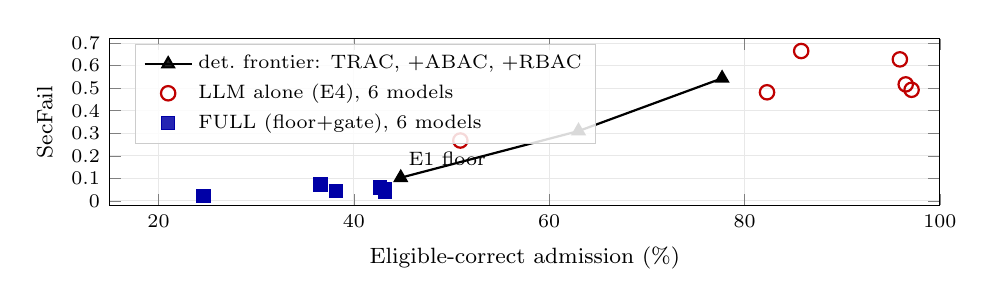
\begin{tikzpicture}
\begin{axis}[
    width=\columnwidth, height=3.7cm,
    xlabel={Eligible-correct admission (\%)}, ylabel={SecFail},
    xmin=15, xmax=100, ymin=-0.02, ymax=0.72,
    xtick={20,40,60,80,100}, ytick={0,0.1,0.2,0.3,0.4,0.5,0.6,0.7},
    grid=major, grid style={gray!18},
    tick label style={font=\scriptsize}, label style={font=\footnotesize},
    legend style={font=\scriptsize, at={(0.03,0.97)}, anchor=north west,
                  cells={anchor=west}, fill=white, fill opacity=0.85,
                  text opacity=1, draw=gray!40},
    legend cell align={left},
]
% Deterministic frontier (bundle-only, model-independent): TRAC-only -> +ABAC -> +RBAC (=E1)
\addplot[thick, black, mark=triangle*, mark size=2.4pt]
  coordinates {(77.7,0.544) (63.0,0.310) (44.8,0.103)};
\addlegendentry{det.\ frontier: TRAC, +ABAC, +RBAC}
% LLM alone (E4): 6 models across 3 vendors
\addplot[only marks, mark=o, mark size=2.6pt, red!75!black, thick]
  coordinates {(50.9,0.268) (85.8,0.665) (82.3,0.482) (97.1,0.493) (96.5,0.517) (95.9,0.628)};
\addlegendentry{LLM alone (E4), 6 models}
% FULL = floor + gate: 6 models across 3 vendors
\addplot[only marks, mark=square*, mark size=2.4pt, blue!65!black]
  coordinates {(24.6,0.021) (36.6,0.073) (38.2,0.044) (43.2,0.040) (43.2,0.051) (42.7,0.059)};
\addlegendentry{FULL (floor+gate), 6 models}
\node[font=\scriptsize, anchor=south west] at (axis cs:44.6,0.115) {E1 floor};
\end{axis}
\end{tikzpicture}
\caption{Operating-point map: SecFail vs.\ eligible-correct admission (fraction of correct candidates admitted; validation). The model-independent deterministic frontier (TRAC $\to$ $+$ABAC $\to$ $+$RBAC) is monotone; every LLM-only (E4) validator sits well above it at high SecFail \emph{regardless} of admission, while composing each model's verdict with the floor (FULL) pulls all six models, across three vendors, into a tight low-SecFail cluster ($\leq7.5\%$), none exceeding the E1 floor. Eligible-correct admission counts \emph{every} denied correct-and-authorised request, including least-privilege denials by RBAC/ABAC; the full stack's over-block on \emph{admissible} requests (the deployment false-block) is $19.3\%$. Values: Table~\ref{tab:stack_guarantee}; replay via \texttt{scripts/sweep\_op\_points.py}.}
\Description{Scatter plot of SecFail against eligible-correct admission. The deterministic policy frontier descends as TRAC, ABAC, and RBAC are added; LLM-only points sit above it at high SecFail, while full-pipeline points cluster near low SecFail at the secure end.}
\label{fig:operating_sweep}
\end{figure}

The deterministic layers trace a \emph{monotone} frontier (each layer lowers SecFail: $54\%\!\to\!31\%\!\to\!10\%$); every LLM-only (E4) point sits well above it regardless of admission, while composing the model behind the floor (FULL) collapses all six models across three vendors into a tight secure cluster ($\leq7.5\%$), none exceeding the E1 floor (\S\ref{sec:reversal}).

\textbf{The security/availability trade-off.} The full stack's eligible-correct admission---$44.8\%$ of correct candidates---is deliberately conservative, but the face value overstates the availability cost because it counts \emph{every} denied correct bundle, including ones a correct agent \emph{should} not be allowed to run. Of the $55.2$pp it does not admit, $44.5$pp are correct-but-\emph{unauthorised} bundles that RBAC/ABAC deny by least privilege (over-privileged or out-of-grant tool use---enforcement working as intended, not a false block); only $10.7$pp are genuine over-blocks of \emph{admissible} (correct \emph{and} authorised) work by the leak-free task-relational layer---the $19.3\%$ deployment false-block. That residual is an \emph{inference} cost and the operating point is tunable (\S\ref{sec:policy_dependence}). The low admission is therefore a deliberate max-security operating point on a policy-navigable frontier, not a fixed limitation.

\subsection{Substrate Portability: Verified OPA/Rego Parity}
\label{sec:substrate_portability}

The guarantee is a property of the \emph{policy}, not our particular engine. PALADIN's RBAC, ABAC, and TRAC layers are authored as \emph{rules-as-data}: the same YAML documents (\texttt{policies/\{rbac,abac\_rules,trac\_rules\}.yaml}) are evaluated both by our reference Python engine and, \emph{unchanged}, by generic Rego policies on a standard Open Policy Agent runtime (OPA v1.18.0). Editing a rule updates both; no code is generated or hand-synced. We verify decision equivalence with the real \texttt{opa} binary: across $120$ RBAC, $120$ ABAC, and $100$ unique-bundle TRAC evaluations, OPA reproduces \emph{every} ALLOW/DENY decision and every advisory of the reference engine---zero mismatches. Parity holds by construction (both evaluate the identical rule data under the same operator semantics) and is confirmed empirically; the same policies also serve from a live \texttt{opa run --server} instance queried over OPA's REST Data API. The portable boundary is the rule-evaluation layer (S3/S4/S6, \S\ref{sec:framework}); the fact transformer (S5---BM25 domain inference and VerbNet action classification) runs once upstream and supplies both engines the same typed predicates. This is a \emph{deployability} result (\S\ref{sec:trac}): the engine is a commodity, so the task-relational policy is enforceable on standard infrastructure---the artefact is the policy and its predicate, not a new runtime. Benchmarking the \emph{performance} cost of the OPA substrate is the remaining follow-up (\S\ref{sec:future_work}).

\subsection{Independent Replication of ASTRA's LLM-ResM Benchmark}
\label{sec:astra_replication}

Under Convention~B (ASTRA permissivity view), our gpt-4o E4 reaches $F_1=0.595$ vs.\ ASTRA's published $0.67$---a $0.075$ gap under a strictly harder protocol (ASTRA AND-aggregates three per-tool verdicts, inflating precision; we use one per-bundle call), so our number is the expected lower bound. The precision--recall signature replicates: high precision ($0.740$ vs.\ $0.81$), low recall ($0.497$ vs.\ $0.57$), under-scoping dominant; the two other panel models bracket gpt-4o ($0.756$, $0.688$). A reproduction of ASTRA's under-scoping finding, not a refutation.

\subsection{Non-Monotone LLM-Only Behaviour with Model Recency}
\label{sec:newer_not_better}

A clean side-effect of the three OpenAI generations: LLM-only (E4) safety is \emph{non-monotone} in recency under \emph{both} conventions (the ordering differs). Under Convention~B ($F_1$), gpt-3.5-turbo-16k (2023, $0.756$) beats gpt-4o (2024, $0.595$) and gpt-5.4 (2026, $0.688$); under Convention~A, gpt-4o is strongest yet the 2026 gpt-5.4 is the \emph{most} permissive (SecFail $0.665$ vs.\ $0.268$). We cannot causally attribute this without a controlled fine-tune, but the lesson holds across vendors---every $2026$ model is a \emph{more} permissive validator than the 2023 one (\S\ref{sec:cross_vendor})---so \emph{a single-LLM validator cannot be assumed to improve as base models advance}.

\subsection{Which Layers Are Load-Bearing: RBAC and TRAC Carry the Load}
\label{sec:reversal}

\begin{table}[!t]
\centering
\caption{Full-factorial layer ablation on the deterministic stack (validation, Convention~A, $n=6{,}942$; model-independent). \textbf{SecFail} lower is safer; \textbf{$\Delta$SecFail} $=$ SecFail $-$ SecFail(full). \emph{Every} ablation is worse on SecFail than the full stack: conventional access control alone (RBAC$+$ABAC, no task-relational layer) leaves SecFail at $0.223$---more than double $0.103$, the operating point of any conventional AC method without the predicate (\S\ref{sec:access_control}). For two-layer rows $\Delta$SecFail equals the omitted layer's drop-one marginal in magnitude (\S\ref{sec:reversal} reports it signed, $<\!0$). Availability and the E4/FULL points: Table~\ref{tab:stack_guarantee}.}
\label{tab:factorial_ablation}
\footnotesize
\setlength{\tabcolsep}{6pt}
\begin{adjustbox}{max width=\columnwidth}
\begin{tabular}{@{}lccc@{}}
\toprule
\textbf{Configuration} & $\mathbf{F_1}$ & \textbf{SecFail} & $\mathbf{\Delta}$\textbf{SecFail} \\
\midrule
No policy (all open)             & 0.000 & 1.000 & $+0.897$ \\
\addlinespace[2pt]
RBAC only                        & 0.793 & 0.242 & $+0.139$ \\
TRAC only                        & 0.591 & 0.544 & $+0.441$ \\
ABAC only                        & 0.532 & 0.610 & $+0.507$ \\
\addlinespace[2pt]
RBAC$+$TRAC \textit{($-$ABAC)}   & 0.850 & 0.112 & $+0.009$ \\
RBAC$+$ABAC \textit{($-$TRAC)}   & 0.795 & 0.223 & $+0.120$ \\
ABAC$+$TRAC \textit{($-$RBAC)}   & 0.751 & 0.310 & $+0.207$ \\
\midrule
\textbf{RBAC\,$\wedge$\,ABAC\,$\wedge$\,TRAC (full)} & 0.848 & \textbf{0.103} & --- \\
\bottomrule
\end{tabular}
\end{adjustbox}
\end{table}

\begin{figure}[!t]
\centering
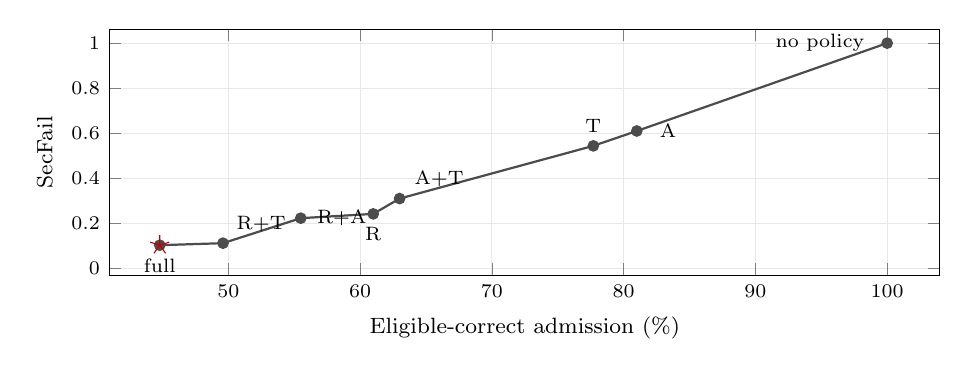
\begin{tikzpicture}
\begin{axis}[
    width=\columnwidth, height=4.7cm,
    xlabel={Eligible-correct admission (\%)}, ylabel={SecFail},
    xmin=41, xmax=104, ymin=-0.03, ymax=1.06,
    xtick={50,60,70,80,90,100}, ytick={0,0.2,0.4,0.6,0.8,1.0},
    grid=major, grid style={gray!18},
    tick label style={font=\scriptsize}, label style={font=\footnotesize},
]
% Deterministic ablation frontier: all eight layer subsets, monotone in admission.
\addplot[thick, black!70, mark=*, mark size=1.7pt]
  coordinates {(44.8,0.103) (49.6,0.112) (55.5,0.223) (61.0,0.242)
               (63.0,0.310) (77.7,0.544) (81.0,0.610) (100.0,1.000)};
% Full stack highlighted.
\addplot[only marks, mark=star, mark size=3.6pt, red!75!black]
  coordinates {(44.8,0.103)};
\node[font=\scriptsize, anchor=north]      at (axis cs:44.8,0.086) {full};
\node[font=\scriptsize, anchor=south west] at (axis cs:49.9,0.118) {R$+$T};
\node[font=\scriptsize, anchor=west]       at (axis cs:56.0,0.223) {R$+$A};
\node[font=\scriptsize, anchor=north]      at (axis cs:61.0,0.228) {R};
\node[font=\scriptsize, anchor=south west] at (axis cs:63.4,0.320) {A$+$T};
\node[font=\scriptsize, anchor=south]      at (axis cs:77.7,0.560) {T};
\node[font=\scriptsize, anchor=west]       at (axis cs:82.0,0.610) {A};
\node[font=\scriptsize, anchor=east]       at (axis cs:99.0,1.000) {no policy};
\end{axis}
\end{tikzpicture}
\caption{Ablation operating points: SecFail vs.\ eligible-correct admission for all eight subsets of the deterministic stack (validation; model-independent; R\,$=$\,RBAC, A\,$=$\,ABAC, T\,$=$\,TRAC). Adding a layer lowers SecFail at an admission cost, tracing a monotone frontier with the full stack (star) at the secure end (SecFail\,$0.103$). Most of the admission gap is correct-but-\emph{unauthorised} least-privilege denial, not false block---the over-block on \emph{admissible} work is $19.3\%$ (\S\ref{sec:operating_sweep}). Values: Table~\ref{tab:factorial_ablation}.}
\Description{Scatter plot with a connecting line showing SecFail against eligible-correct admission for all eight layer subsets. As layers are added, admission decreases and SecFail decreases monotonically, with the full RBAC-ABAC-TRAC stack at the low-admission, low-SecFail secure end and the no-policy baseline at full admission and SecFail one.}
\label{fig:ablation_frontier}
\end{figure}

Table~\ref{tab:factorial_ablation} scores all eight subsets of the deterministic stack (validation; deterministic, hence model-independent): \emph{every} ablation is strictly worse on SecFail than the full stack, and conventional access control alone---RBAC$+$ABAC with no task-relational layer---leaves SecFail at $0.223$, more than double the full stack's $0.103$ (frontier in Fig.~\ref{fig:ablation_frontier}). We read each layer's contribution two ways. The order-dependent \emph{successive} deltas (E1$\to$E2$\to$E3) are large for every layer---removing RBAC first raises validation SecFail $20.7$pp, then removing ABAC a further $23.4$pp, leaving the TRAC-only floor at $54\%$ (selection is larger still, TRAC-only $75\%$). But the honest per-layer measure is the order-independent \emph{drop-one} marginal (SecFail of the full stack vs.\ the stack with exactly that one layer removed). Here the picture sharpens: RBAC ($-20.7$pp, $95\%$ CI $[-22.6,-19.0]$) and \textbf{TRAC ($-12.0$pp, $[-13.5,-10.6]$)} are each individually load-bearing---both CIs exclude $0$---whereas \textbf{ABAC's drop-one marginal is only $-0.9$pp} ($[-1.3,-0.6]$)---because ABAC and RBAC \emph{overlap}: most attribute violations ABAC would catch are already caught by RBAC. ABAC is therefore a \emph{backstop}: near-redundant given RBAC on this benchmark, but load-bearing when RBAC is absent (its $-23.4$pp successive delta is exactly that regime).

Two readings follow. TRAC's isolated $-12.0$pp is direct evidence the task-relational axis catches violations conventional RBAC$+$ABAC cannot---measured, not asserted. And the successive-vs.-drop-one gap for ABAC instances the attribution pitfall of \S\ref{sec:attribution_paradox}: a layer can look essential under one convention and near-redundant under another, so both must be reported---guidance not ``never drop a layer'' but ``RBAC and TRAC are individually load-bearing; ABAC hedges RBAC.'' This also corrects the earlier oracle-aided policy, in which an alignment score did most of the validation work and RBAC/ABAC were near-redundant; removing the oracle redistributes the security load onto identity and the task-relational predicate---exactly where a zero-trust deployment can audit it.

\textbf{Is the load-bearing pattern a label artefact?} Two decouplings say no. Re-authoring RBAC \emph{independently} of the label (coarse job-function roles that \emph{over-provision} relative to the fine-grained allow-list) shrinks RBAC's drop-one marginal ($-20.7\!\to\!-11.3$pp), but the slack redistributes onto TRAC ($-12.0\!\to\!-21.5$pp) and ABAC ($-0.9\!\to\!-9.1$pp) and the floor degrades gracefully (SecFail $10.3\!\to\!19.7\%$) while admitting strictly more legitimate work---no single layer's exact tuning is load-bearing. Decoupling the \emph{label} itself from all policy (legitimacy from ASTRA's \texttt{match\_tag} alone, dropping the persona--domain criterion) makes \textbf{TRAC's marginal \emph{rise} to $-17.2$pp $[-19.1,-15.5]$, the largest of the three} (paired task-level bootstrap $95\%$ CI clear of $0$; RBAC falls to $-14.6$pp $[-16.5,-12.7]$): under a label no policy artefact authored, the task-relational predicate is the \emph{most} load-bearing layer---the opposite of a circularity artefact.

\textbf{Is TRAC informative, or just more denials?} On the RBAC$\wedge$ABAC-approved set ($2{,}206$ bundles, $\approx$half illegitimate, where only a task-relational signal discriminates), a \emph{volume-matched random denier} catches $\approx\!406$ violations and blocks $\approx\!403$ legitimate; TRAC, at the same volume, catches $597$ and blocks only $212$ (precision $0.74$ vs.\ base rate $0.50$)---the marginal is signal, not added volume.

\textbf{The enforcing surface is not only lexical.} Two TRAC rules reason about \emph{action semantics}: \texttt{action\_coherence} (read-intent task, mutating tools) and \texttt{write\_safety} (destructive op without a preceding read). Making \texttt{action\_coherence} enforcing catches $39$ same-domain violations the BM25 predicates and RBAC$+$ABAC all miss, at precision $0.62$ ($1.69\times$ the approved base rate), lowering SecFail $10.3\!\to\!9.5\%$ at $24$ new legitimate blocks---structural coherence beyond BM25. (\texttt{write\_safety} is weaker, precision $0.31$, so advisory.)

\subsection{The Attribution Paradox}
\label{sec:per_domain}
\label{sec:attribution_paradox}

Marginal necessity and first-firing attribution disagree sharply. Attributing every E1 denial to the first layer that fires under short-circuit order (RBAC$\to$ABAC$\to$TRAC), RBAC claims $82\%$ of denials, TRAC $15\%$, and ABAC only $4\%$. Yet the marginal picture (\S\ref{sec:reversal}) is the opposite: ABAC, which first-fires on a mere $4\%$ of denials, carries the largest \emph{successive} marginal ($-23.4$pp---removing ABAC once RBAC is already absent), even though its order-independent \emph{drop-one} marginal is only $-0.9$pp. The reason is pipeline order---most rows ABAC would catch are intercepted earlier by RBAC, so ABAC's unique value is invisible to a denial-source chart and surfaces only when RBAC is removed. First-firing attribution, common in the agent-safety literature, therefore systematically misranks layers; both attribution and marginal $\Delta\mathrm{SecFail}$ must be reported.

\subsection{Corroborated Coverage}
\label{sec:corroborated}

The leak-free domain classifier (\S\ref{sec:domain_inference}) is intentionally imperfect: a business-phrased task can route to a lexically-similar but wrong MCP, so \texttt{capability\_coverage} occasionally denies a correct, in-domain bundle. \emph{Corroborated coverage} reverses such a denial when an \emph{independent} signal---the mean BM25 relevance of the selected tools to the task---is high ($\geq\!4.0$): a legitimate, domain-mis-routed bundle still has tools that lexically match the task, whereas a genuinely wrong-domain bundle does not. Over the model-independent validation profile, enabling the rescue cuts TRAC's unique over-denials of legitimate work from $233$ to $212$, at a cost of $+0.08$pp SecFail and four lost catches---a small Pareto refinement (the sweep knee is $4.0$) that reintroduces no oracle.

\subsection{Dataset Ceiling and Post-Hoc Enforcement}
\label{sec:ceiling}

Selection exact-match is intrinsically low ($11.4\%$ baseline): tool-naming pedantry over $194$ non-standardised identifiers, multiple defensible bundles scored against one gold, cross-persona ambiguity, and a brittle all-or-nothing match cap it independently of model capability. Conservatively the practical ceiling is $30$--$40\%$; Jaccard is the less-misleading signal.

\textbf{Post-hoc enforcement.} In selection mode the deterministic stack does not alter the LLM's selections: tool exact-match and Jaccard are recorded per row \emph{before} policy gating, so the E1$\to$E3 SecFail differences are purely policy-attributable---PALADIN is a true post-hoc enforcement layer.

%==============================================================================
% SECTION 9: DISCUSSION
%==============================================================================
\FloatBarrier
\section{Discussion}
\label{sec:discussion}

\subsection{Operating Point, Policy Dependence, and Generalisability}
\label{sec:deployment_envelope}
\label{sec:policy_dependence}

The floor's $19.3\%$ false-block is an \emph{inference} cost (\S\ref{sec:operating_sweep}): it comes entirely from the two BM25 predicates (\path{capability_coverage}, $160$; \path{tool_relevance}, $52$)---RBAC and ABAC deny no admissible request by construction---and an \emph{oracle} domain lowers it to $14.0\%$ ($\sim\!5$pp router error, $\sim\!14$pp genuine lexical sparsity, recoverable with a stronger retriever). Nor is the floor fixed: three knobs in \texttt{policies/trac\_rules.yaml} (the \texttt{capability\_coverage} floor, the \texttt{tool\_relevance} cutoff, the rescue bar) and the choice of enforcing layers navigate the frontier (Fig.~\ref{fig:operating_sweep})---TRAC \emph{advisory} at SecFail $22.3\%$, an over-provisioned RBAC (\S\ref{sec:reversal}) at $19.7\%$---so we recommend advisory-TRAC as an availability-balanced default and the full floor where security is paramount (\S\ref{sec:future_work}).

\textbf{Generalisation across tool catalogs.} With one fixed operating point (no per-domain tuning), across ASTRA's eight MCP domains (distinct tool catalogs) the floor holds $F_1\in[0.78,0.89]$ (sd $0.033$)---not overfit to one distribution; SecFail spans $0$--$21\%$ by domain and admissible false-block $0$--$63\%$ (\texttt{wikipedia}, a $10$-tool catalog, the outlier). Worst-group holds: in \emph{every} catalog the model-independent floor's SecFail lies below \emph{every} OpenAI generation's E4 SecFail---per-catalog, not aggregate. So the fixed thresholds are robust \emph{across catalogs within} ASTRA's construction; certifying the signal \emph{beyond} it needs an independently-labelled or second corpus (\S\ref{sec:future_work}).

The guarantee is conditional on the authored policy but bounded: removing any denial rule cannot decrease SecFail (short-circuit), so the per-layer marginals (\S\ref{sec:reversal}) upper-bound the damage from disabling a rule family.

\subsection{The Floor's Adversarial Limit, Quantified}
\label{sec:adversarial}
Our threat model (\S\ref{sec:threat_model}) assumes trusted task provenance---the operator authors the task; the agent proposes only the \emph{bundle}---but we stress-test its violation, which few enforcement papers do. Giving an adversary the task text and appending the bundle's \emph{own} tool names and descriptions (naive prompt-injection-style padding) collapses TRAC's catch on the $578$ bundles it targets from $57.1\%$ to $0.0\%$. Is this specific to the lexical BM25 predicates? We re-instantiate both enforcing predicates with a deterministic local semantic embedding (model2vec, no API): it catches \emph{more} clean ($57.1\!\to\!70.9\%$) yet is \emph{equally} defeated by padding ($70.9\!\to\!4.8\%$). The attack poisons the task text itself, so \emph{no} predicate over that text---lexical or semantic---resists it: the evasion is a property of \emph{untrusted task provenance}, and the control is input integrity (the composed prompt-injection layer, \S\ref{sec:threat_model}), not a stronger relevance function. Within the semi-honest model the guarantee holds; the embedding's higher clean-case catch is an option for deployments willing to trade determinism for a model dependency.

\subsection{Limitations and Threats to Validity}
\label{sec:limitations}

Table~\ref{tab:threats} summarises the dominant threats to validity---internal, external, construct, and statistical---each with its mitigation and a pointer to the relevant section or released artefact.

\begin{table}[!t]
\centering
\caption{Threats to validity at a glance. Mitigations link back to the indicated section or released artefact.}
\label{tab:threats}
\scriptsize
\setlength{\tabcolsep}{3pt}
\begin{tabularx}{\columnwidth}{@{}>{\raggedright\arraybackslash}p{1.8cm}>{\raggedright\arraybackslash}X@{}}
\toprule
\textbf{Category} & \textbf{Threat \& mitigation} \\
\midrule
\multicolumn{2}{@{}l}{\textit{Internal}} \\
Pipeline ordering & Layer attribution conditioned on RBAC$\to$ABAC$\to$TRAC; per-layer marginals are ordering-independent (\S\ref{sec:reversal}). \\
Implementation bugs & Raw per-row logs for every reported run and analysis scripts released; ASTRA replication cross-validates the verdict path against an external baseline (\S\ref{sec:astra_replication}). \\
\midrule
\multicolumn{2}{@{}l}{\textit{External}} \\
Vendor coverage & Three OpenAI generations $+$ a full blind non-OpenAI panel (Claude Opus 4.8, Claude Sonnet 4.6, Gemini 2.5 Pro; $n\!=\!6{,}942$ each, \S\ref{sec:cross_vendor}); open-weights (Llama, Mistral) deferred (\S\ref{sec:future_work}). \\
Dataset & ASTRA v0.3 is, to our knowledge, the only public corpus with the required label structure (\S\ref{sec:dataset}); single-source risk is mitigated by fixed-threshold generalisation across its $8$ tool catalogs ($F_1\!\in\![0.78,0.89]$, \S\ref{sec:deployment_envelope}). A structurally comparable second corpus is future work. \\
\midrule
\multicolumn{2}{@{}l}{\textit{Construct}} \\
Per-bundle vs.\ per-tool & Our E4 is one LLM call per bundle; ASTRA LLM-ResM is per-tool with AND-aggregation---disclosed, consistent with the $0.075$ $F_1$ gap direction (\S\ref{sec:astra_replication}). \\
Convention conflation & Two conventions documented (\S\ref{sec:conventions}); every table flags which applies. \\
Adversarial task text & Task-text predicates (lexical \emph{and} semantic---we test both, \S\ref{sec:adversarial}) are evaded by adversary-crafted task text; out of scope by construction (trusted provenance, \S\ref{sec:threat_model}), the defence is input integrity via composed prompt-injection controls~\cite{liu2024formalizing}. \\
\midrule
\multicolumn{2}{@{}l}{\textit{Statistical}} \\
Layer marginals & Paired task-level bootstrap $95\%$ CIs ($1{,}000$ resamples); per-model and per-domain agreement provide robustness checks. \\
Policy dependence & Per-layer $\Delta\mathrm{SecFail}$ upper-bounds damage of silently disabling a rule family; controlled perturbation study deferred (\S\ref{sec:future_work}). \\
Domain inference & Task domain inferred from task text by BM25, consuming \emph{no} ground-truth label (\S\ref{sec:domain_inference}); an earlier \texttt{gt\_mcps[0]} stand-in is removed, so both modes are leak-free. The $\sim\!60$--$70\%$ top-1 accuracy is the honest cost, mitigated by corroborated coverage (\S\ref{sec:corroborated}). \\
\bottomrule
\end{tabularx}
\end{table}

\subsection{Future Work and Artifact Availability}
\label{sec:future_work}
\label{sec:artifacts}

With full Anthropic and Google panels now reported (\S\ref{sec:cross_vendor}), the remaining cross-vendor extension is an \textbf{open-weights panel} (Llama, Mistral) beyond the three OpenAI generations and the two commercial non-OpenAI vendors. Computable from the released artefact without new LLM calls: a \textbf{Cedar port and OPA/Rego performance benchmark} (decision parity is already shown, \S\ref{sec:substrate_portability}; only latency/throughput cost is open), a \textbf{policy-perturbation sensitivity study} restricted to predicate-removal ablations, a \textbf{continuous threshold-grid sweep} over the three exposed TRAC knobs mapping the full SecFail/false-block surface. Requiring new LLM calls: a selection-mode LLM-on-LLM-bundles baseline (\S\ref{sec:reversal}), \textbf{active adversarial inputs} beyond ASTRA's \texttt{wrong}/\texttt{null} model, a \textbf{second adversarial dataset}~\cite{zhan2024injecagent,debenedetti2024agentdojo,ruan2024toolemu}, \textbf{argument- and resource-instance-level authorisation} (beyond the tool-bundle granularity modelled here), and \textbf{multi-hop tool chains}.

We release the complete PALADIN implementation as open-source software.\footnote{Anonymous repository for review: \url{https://anonymous.4open.science/r/paladin-sacmat2027/}; the original repository name describes the policy-stack components and will be renamed for the camera-ready.} The release includes the pipeline source; all policy configurations; 8 MCP server tool definitions ($194$ tools); the ASTRA v0.3 dataset; raw per-row logs for the reported runs (six validation runs across three vendors and a selection baseline); analysis scripts regenerating every number; and a Dockerised runner with configurable ablations. (The released \path{policies/} retains legacy oracle-path files---e.g.\ \path{domain_capability_*.json}---not read by the evaluated agnostic pipeline.) \emph{Citation hygiene:} recent or in-press references~\cite{gupta2025security,jamshidi2025securing,chu2026stateless,patil2026sentinelagent,rampalli2026pedigree} are concurrent or near-concurrent work; none share authorship with this submission to the best of our knowledge.

%==============================================================================
% SECTION 10: CONCLUSION
%==============================================================================
\section{Conclusion}
\label{sec:conclusion}

Autonomous agents have turned the tool-invocation boundary into a security surface the Model Context Protocol leaves ungoverned, and the prevailing question---\emph{is the model safe?}---is the wrong one. A model's unaided judgment is neither stable nor monotone in capability: across our panel, ungoverned tool admission ranges from a competent validator (gpt-4o, E4 $F_1=0.760$) to a near-yes-machine that lets two-thirds of mis-scoped bundles through (gpt-5.4, E4 SecFail $=0.665$)---an $F_1$ span of $0.28$ with no ordering by model recency. The operative question is what must be enforced \emph{before} the call, regardless of which model authored the request---and our central result is that a thin \emph{deterministic} admission layer answers it, holding SecFail to a fixed $10.3\%$ ($F_1$ $0.848$) identically across every model. The guarantee is a property of the stack, not the LLM.

Our measurement framework is built to show this rather than assert it. By separating what the model contributes from what the policy contributes---through dual-mode evaluation and two explicit metric conventions---it makes the masking effect measurable, and in doing so surfaces structure prior task-tool benchmarks could not: three deterministic layers of differing marginal weight (RBAC and TRAC individually load-bearing, ABAC a backstop), first-firing attribution that overstates upstream necessity while hiding ABAC's necessity when RBAC is absent, and a retrieval intervention that improves accuracy and security together. PALADIN contributes a task-relational admission primitive within a security-first floor---not a complete new access-control model, nor an end-to-end agent-safety solution. Its lesson for the agentic era is a single design principle: authorisation must not ride on model trustworthiness. Determinism, not capability, is what turns an unpredictable model into a predictable security surface.

%==============================================================================
% REFERENCES
%==============================================================================
\bibliographystyle{ACM-Reference-Format}
\bibliography{references}

\end{document}

